\label{sec:problem}
%\textbf{Robot and Environment Model. } 
The robot perceives the world state comprising a set of rigid objects placed on a table via a depth sensor that outputs a depth image $S \in \real^{H\times W \times C}$, where $H,W,C$ respectively
%. Here, the superscript 
denote the height, width and the number of channels (including depth) of the imaging sensor.  
%
% Further, the robot's perception system includes object detector that can identify object proposals and determine bounding boxes for 
% object instances detected in the environment.  
%
% Let $b_{i} \in \real^{4}$ represent a bounding box 
% for the $i^{th}$ object represented with two 2D coordinates of the diagonal end-points.
%
% Finally, the data association between observed bounding boxes and object instances is assumed known in images across time.  
% %
The workspace is co-habited by a human partner 
who provides language instructions 
%for robot to perform assembly tasks with instructions such as  
% such as
% \emph{``put the small green block to left of yellow lego block"} etc. 
%
to the robot to perform assembly tasks.
We assume a closed world setting, i.e. changes to the world state are caused only by the robot manipulator. 

%\textbf{Language-guided Task Execution. }
The robot's goal is to interpret the human's instruction $\Lambda$ 
in the context of the initial world state $S_I$ and determine a 
sequence of low-level  motions that result in the final world state 
$S_F$ conforming to the human's intention.  
%
%Performing an instructed task can involve complex interactions requiring 
%an extended sequence of low-level motions to perform a long-horizon 
%objective (e.g., completing a stack assembly of blocks). 
%
Following ~\cite{kaelbling2010hierarchical, zhu2020hierarchical}, 
planning for a complex task is factorized into  (i) high-level task planning to determine a sequence of sub-goals, and (ii) the generation of 
low-level motions to attain each sub-goal. 
%
Formally, a semantic model for a manipulation task denoted as $ManipulationProgram(.)$ takes the initial scene $S_I$ and the instruction $\Lambda$ as input and determines a sequence of 
sub-goals as $(g_0, g_1, \dots, g_n) = ManipulationProgram(S_I, \Lambda)$. 
%
Each sub-goal $g_i$ aggregates the 
knowledge of the object, $o_i$, to be manipulated 
and its target Cartesian $SE(3)$ pose $p_i$. This is  
provided to the low-level motion planner 
to synthesize the end-effector trajectory for the robot to execute. 
%
The robot's motion planner, which is assumed to be given, includes grasping an object  
and synthesizing a collision-free trajectory for positioning it at a target pose. 
%
% Online, when the robot is instructed, it uses the learned model to 
% interpret the instruction as per the current world state and 
% predicts sub-goals which are then sequentially attained. 
%in the environment.  
%


%This paper addresses the problem of learning the task planning model introduced above. 
%
% Let the task planning model be realized as a function parameterized with trainable parameters $\Theta$.  
%
%During training, we assume that 
Training data consists of demonstrations, corresponding to task instructions $\Lambda$, in the form of initial 
and final 
world states $(S_I, S_F)$.
%
Given data $D$$=$$\{ S^{i}_I, S^{i}_F, \Lambda^{i} \}^{M}_{i=1}$, the model parameters are trained by optimizing a loss 
$\mathcal{L}(\tilde{S}_F^{i},S_F^{i})$
%
%\begin{equation*}
%     \sum_{i}^{M}\mathcal{L}(S_I^{i} = Execution(TaskPlanner(S_I^{i}, \Lambda)), S_F^{i}; \Theta),      
%\end{equation*}
where 
\begin{equation}
\tilde{S}_F^{i}=Simulate(ManipulationProgram(S_I^{i}, \Lambda; \Theta))
\end{equation} is the final state estimated by simulating the plan inferred by $ManipulationProgram(S_I^{i}, \Lambda)$ on initial state $S_I^i$. (figure \ref{fig:problem-1}) 
%\textcolor{red}{Shouldn't loss take plan emitted by task planner (or task planer) as input, or it can be written as %$\mathcal{L}(Plan = TaskPlanner(S_I, \Lambda), S_F; \Theta)$}
% 
We seek strong generalization on novel scenes, instructions and plan lengths 
beyond those encountered during training, along with interpretability in sub-goals. 

\begin{figure}
    \centering
    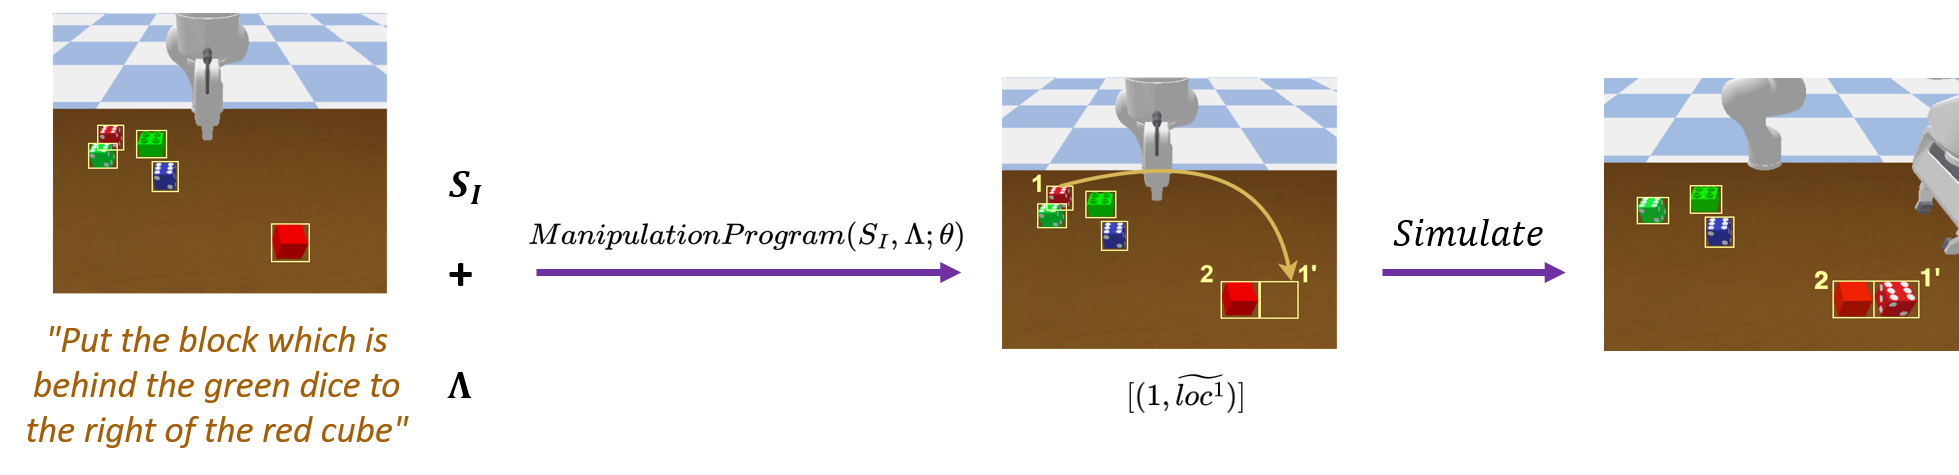
\includegraphics[width=\textwidth]{assets/part1-problem.png}
    \caption{Problem formulation: Learning robot manipulation programs}
    \label{fig:problem-1}
\end{figure}